\documentclass[11pt,a4paper]{article}
\usepackage[margin=24mm]{geometry}
\usepackage[T1]{fontenc}
\usepackage{lmodern}
\usepackage{amsmath,amssymb,booktabs,longtable,array,graphicx,pdflscape}
\usepackage{enumitem,xcolor,tikz}
\usetikzlibrary{arrows.meta,positioning}
\usepackage{microtype}
\usepackage[colorlinks=true,linkcolor=blue!45!black,citecolor=blue!45!black,urlcolor=blue!45!black]{hyperref}
\usepackage{xurl}
\setlength{\emergencystretch}{2em}
\setlength{\parskip}{4pt}
\setlength{\parindent}{0pt}
\newcolumntype{P}[1]{>{\raggedright\arraybackslash}p{#1}}
\setlist{nosep,leftmargin=*}
\setcounter{tocdepth}{1}
\newcommand{\code}[1]{\nolinkurl{#1}}
\newcommand{\runid}{\code{evaluation_20261012T040605_929193Z}}
\newcommand{\na}{\textemdash}
\title{CPU-Only Screening of CLIP and Generative Vision--Language Models for Surveillance Anomaly Detection:\\Methods, Experimental Evidence, and Limits of a Four-Model Study}
\author{Capstone anomaly detection project\\Technical report derived from recorded experiment artifacts}
\date{12 October 2026}

\begin{document}
\maketitle
\begin{abstract}
Selecting an anomaly detector for a CPU-only, approximately 32\,GB, single-camera deployment requires separate evidence of event discrimination and computational feasibility. This report reconstructs and audits a four-model experiment involving MobileCLIP2-S2, SigLIP2-B/16-224, SmolVLM-500M-Instruct and MiniCPM-V 4.0. The prepared evaluation contains 236 historical smoking development frames and 72 CAVIAR image inputs, comprising endpoint and past-window representations of the same 36 labeled moments. Execution used CPU float32 inference, 32 threads, three repeats, pinned checkpoints and common task-specific cohorts. Of 3,696 planned measured predictions, 3,684 were saved; nineteen of twenty model/cohort jobs completed. MiniCPM's smoking job exceeded its one-hour timeout during the third repeat. Recomputed classification metrics, calibration and saved bootstrap outputs agree with the complete artifacts. On sixteen unattended-item test endpoints, three models always predict normal and SmolVLM always predicts the event. Past-window inputs give MobileCLIP event F1 of 0.250 and SmolVLM F1 of 0.353, compared with 0.400 for an always-event baseline. Development-calibrated MobileCLIP endpoint recall reaches 1.000 with a false-positive rate of 0.667; low-FPR thresholds have zero test event recall. CLIP test p95 latency is approximately 0.044--0.065\,s, whereas the generative models require approximately 2.73--5.37\,s on the recorded Threadripper server. Three requested anomalies remain untested, smoking lacks an untouched test set, and CAVIAR has one positive recording per split. The evidence supports a reproducible exploratory screening report and diagnosis of failure modes. It does not establish a five-event deployment winner or performance on the intended Ryzen AI Max+ 395-class host.
\end{abstract}

\newpage
\begingroup\small\tableofcontents\endgroup
\newpage

\section{Objective, research questions and scope}
The project seeks to recognize smoking, loitering, littering, unattended personal items and rough sleeping from camera imagery under a CPU-only deployment constraint. The intended deployment configuration is approximately 32\,GB RAM, or slightly more, with one camera stream initially. A Ryzen AI Max+ 395-class machine is the target discussed in the project. This experiment instead measures a substantially larger computation server. These are distinct hardware settings and are kept separate throughout the analysis.

The immediate scientific question is whether pretrained image--text models can discriminate the defined events, and whether their resource costs justify further adaptation. The experiment tests a common binary interface for each available event: \code{normal} versus that event. It does not run a five-class classifier, a multi-label detector, object tracking or an alert-generating camera service. \code{normal} means negative for the task being evaluated; a not-smoking label is not evidence that every other anomaly is absent.

Three questions structure the report:
\begin{enumerate}
\item Which pretrained candidates distinguish available event examples from task-specific controls using the implemented prompts and image policies?
\item Does adding a short, chronological past-window image representation improve this discrimination relative to its paired endpoint frame?
\item What inference latency, throughput, memory use and output reliability are observed on the measured CPU host, and what remains necessary for a deployment decision?
\end{enumerate}
The strongest supported answer is a screening conclusion, not a general model ranking. All four models were requested, but the smoking experiment is partially incomplete; only unattended items have development/test support. Missing evaluations are explicitly absent, rather than assigned zero accuracy or combined into a weighted winner score.

\subsection{Evidence hierarchy and documented rationale}
Numerical claims in this report are derived from \runid, principally \code{evaluation.json}, cohort \code{run.json}, model \code{summary.json}, \code{predictions.jsonl}, \code{calibration.json}, \code{improvements.json} and logs. The source implementation is available in \code{anomaly_eval/}; all 28 recorded Python/configuration hashes match the inspected checkout. The thin notebook invokes this same runner and does not supply an independent experiment or additional measurements.

The report distinguishes recorded settings, rationales directly supported by comments and configurations, interpretation of observed behavior, and proposed future experiments. Reasons such as controlling correlated examples, preserving scene boundaries and separating threshold tuning from test scoring are justified by the implemented design. The artifact folder does not contain a preregistration or a complete decision diary. Consequently, the report does not claim that undocumented prompt searches, rejected checkpoints or manual labeling procedures occurred.

\section{Model families and shortlist rationale}
CLIP introduced transferable visual representations through paired image/text supervision and similarity-based zero-shot decisions \cite{clip}. The shortlist compares two embedding-based candidates with two generative vision--language candidates. This contrasts relatively inexpensive image encoding and cached text descriptions with autoregressive responses that can, in principle, express uncertainty and contextual judgments. General benchmark performance motivates evaluating a candidate; it does not demonstrate detection of these surveillance events.

MobileCLIP2 improves the reinforced training recipe for compact image--text models \cite{mobilepaper}. The S2 model card reports 35.7\,M image and 63.4\,M text parameters; the implementation uses its canonical OpenCLIP port \cite{mobilecard}. It provides the compact candidate for the CPU resource screen. SigLIP2 extends sigmoid-based image--text pretraining and representation learning \cite{siglippaper,siglip2paper}; the selected base, patch-16, 224-resolution checkpoint provides a second embedding-based reference \cite{siglipcard}. Its scores must retain their independent sigmoid interpretation, rather than be normalized as if they were CLIP softmax probabilities.

SmolVLM is designed as a compact multimodal family \cite{smolpaper}. The selected 500M instruction checkpoint provides a small generative baseline using the publisher's image/text processing and chat template \cite{smolcard}. MiniCPM-V 4.0 is a larger generative comparison: the publisher describes a 4.1\,B model using SigLIP2-400M and MiniCPM4-3B \cite{minicard}. It is included to test whether a larger multimodal model improves task discrimination enough to offset CPU latency and RAM cost. No quantization or alternative serving runtime is evaluated here; publisher device demonstrations therefore cannot be substituted for this float32 benchmark.

\begin{table}[htbp]\centering\small
\caption{Executed checkpoint identifiers and immutable revisions. Names identify the actual artifacts, including the OpenCLIP port.}
\begin{tabular}{p{3.4cm}p{6.4cm}p{5.0cm}}
\toprule Model & Hugging Face identifier & Revision \\ \midrule
MobileCLIP2-S2 & \path{timm/MobileCLIP2-S2-OpenCLIP} & \path{ac6b37c8fc40b62b623d09ed228a6f0c9bc29fe6}\\
SigLIP2-B/16-224 & \path{google/siglip2-base-patch16-224} & \path{75de2d55ec2d0b4efc50b3e9ad70dba96a7b2fa2}\\
SmolVLM-500M & \path{HuggingFaceTB/}\newline\path{SmolVLM-500M-Instruct} & \path{a7da5b986cb59b408707209984f360a5f4ad7e47}\\
MiniCPM-V 4.0 & \path{openbmb/MiniCPM-V-4} & \path{6f69a8235885be89608f3a71ffd40695b379e1e7}\\
\bottomrule\end{tabular}
\label{tab:checkpoints}\end{table}

VadCLIP was shortlisted earlier but was not executed in this run: \code{vadclip=false}, with no adapter, extraction, training or test artifacts. The published method adapts frozen CLIP representations to weakly supervised video anomaly detection \cite{vadclip}. The repository's optional smoking study uses a separately supervised temporal adapter and a different protocol, with frame labels and potentially future session context. It is neither a fifth completed result nor a direct reproduction of the published weakly supervised video experiment. Its omission prevents a complete five-model comparison.

\section{Data sources, definitions and preparation}
\subsection{Operational event definitions}
The configuration defines smoking through a visible smoking object near the mouth or visible smoke. Littering requires a person visibly discarding rubbish on the ground rather than using a bin. Loitering requires remaining in an area over an extended interval without an apparent activity, with temporal evidence. Rough sleeping is framed as apparently sleeping or lying with bedding in a public area; the instruction explicitly limits inference to visible evidence and does not infer housing status. Unattended items require an apparently left-behind personal item without its owner nearby, with evidence of ownership and duration.

The implemented definitions do not specify a universal number of seconds for loitering or abandonment, a distance threshold for an owner, or a validated criterion for sleep. These omissions are material for final event-level evaluation. The CAVIAR configuration supplies a narrower endpoint-state criterion: a carried/deposited bag remains visible after its associated carrier leaves the vicinity; attended placement and retrieval are negative. It explicitly states that this is not a universal duration rule. A six-second sheet supplies past context but cannot validate arbitrary long-duration criteria.

\subsection{Original smoking corpus and historical development policy}
Smoking frames come from the original shared Drive corpus, specifically the smoking-video COCO export. \code{collect_smoking} reads its source \code{train} and \code{valid} annotation files. A frame is positive if it has any \code{Smoking} bounding box, even if \code{Not Smoking} boxes also occur. Otherwise a frame with a \code{Not Smoking} box is a task-specific normal. Frames without either usable category are not included in this collector. Missing files are omitted rather than manufactured as negatives.

The evaluation uses whole images. Annotation boxes determine frame labels but are not used as oracle crops, detector inputs or localization ground truth for scored predictions. COCO source train/valid names do not determine the final evaluation split. Source groups are inferred from filename camera/date patterns, such as \code{smoke:c1:2025-09-11}; this protects camera/day-related imagery from arbitrary frame-level splitting but does not prove every file is an independent recording.

Historically inspected groups are forced into development. This protects against presenting previously examined data as a new untouched test set. The selected smoking cohort has 236 images: 116 positives and 120 task-specific normals in sixteen camera/date groups. Both labels occur in all sixteen groups. Cameras c1, c2 and c4 occur in the recorded names; no new-camera holdout was measured. The sample count is larger than the earlier pilot but still provides development evidence only.

\subsection{CAVIAR state labels and matched controls}
CAVIAR provides staged activity sequences and annotations from its project \cite{caviar}. The scored curated subset uses six named recordings: \code{LeftBag}, \code{LeftBag_AtChair}, \code{LeftBag_PickedUp}, \code{Walk1}, \code{Walk2}, and \code{Walk3}. Nine configured review intervals cover deposited-and-left bags, attended placement, return/pickup, and walking controls. The configuration records review based on sequence XML roles/groups plus chronological frame inspection and recommends independent event-boundary review. This is preliminary annotation review, not a documented blinded multi-rater labeling study.

Each interval yields four equally spaced labeled endpoint times including both boundaries. For a positive interval, preparation requires the nearest XML frame, using a nominal 25\,fps index, to contain a \code{leaving object} role. The preceding visual context is extracted using ffmpeg presentation-time sampling. Explicit interval notes record object/carrier associations. The automatic XML check strengthens annotation consistency but does not alone establish a comprehensive operational ownership rule.

The development split has \code{LeftBag} as the sole positive recording, with \code{LeftBag_PickedUp} and \code{Walk3} as additional controls. The test split has \code{LeftBag_AtChair} as the sole positive recording, with \code{Walk1} and \code{Walk2} as controls. Each positive recording also supplies four attended negatives. Development contains four positive and sixteen normal endpoints; test contains four positive and twelve normal endpoints. The four test positives are moments from one event recording, not four independent positive events.

\begin{table}[htbp]\centering\small
\caption{Prepared and executed coverage. Window and frame rows share labeled CAVIAR endpoint moments and recording splits.}
\setlength{\tabcolsep}{4pt}
\begin{tabular}{llrrrrl}\toprule
Task/input & Split & Event & Normal & Groups & Event groups & Role\\\midrule
Smoking/frame & Dev &116&120&16&16&Historical development\\
Unattended/frame & Dev &4&16&3&1&Preliminary development\\
Unattended/frame & Test &4&12&3&1&Preliminary sequence holdout\\
Unattended/window & Dev &4&16&3&1&Paired past context\\
Unattended/window & Test &4&12&3&1&Paired past context\\
Littering & -- &--&--&--&--&No confirmed cohort\\
Loitering & -- &--&--&--&--&No confirmed cohort\\
Rough sleeping & -- &--&--&--&--&No confirmed cohort\\
\bottomrule\end{tabular}\label{tab:coverage}\end{table}

\subsection{Endpoint and past-window image protocols}
For each time $t$, the frame protocol uses the last image at $t$. The window protocol uses four images at $\max(0,t-6)$, $\max(0,t-4)$, $\max(0,t-2)$ and $t$. They are placed in a $2\times2$ contact sheet in chronological reading order with a 32-pixel header naming that order. No future frame is included relative to $t$. A sheet is one image input to every model, rather than a native video request or four separate inference calls.

This policy gives the embedding and generative adapters access to the same bounded past evidence. It also introduces a representation tradeoff: after common and native resizing, each panel may contain fewer useful pixels than the endpoint alone. Small cigarettes or bags can become difficult to resolve. The present experiment changes the temporal evidence and image layout together; it cannot isolate the effect of time from panel resolution or the text header. The window protocol is also supported only for CAVIAR here, so no smoking window improvement is claimed.

\begin{figure}[htbp]\centering
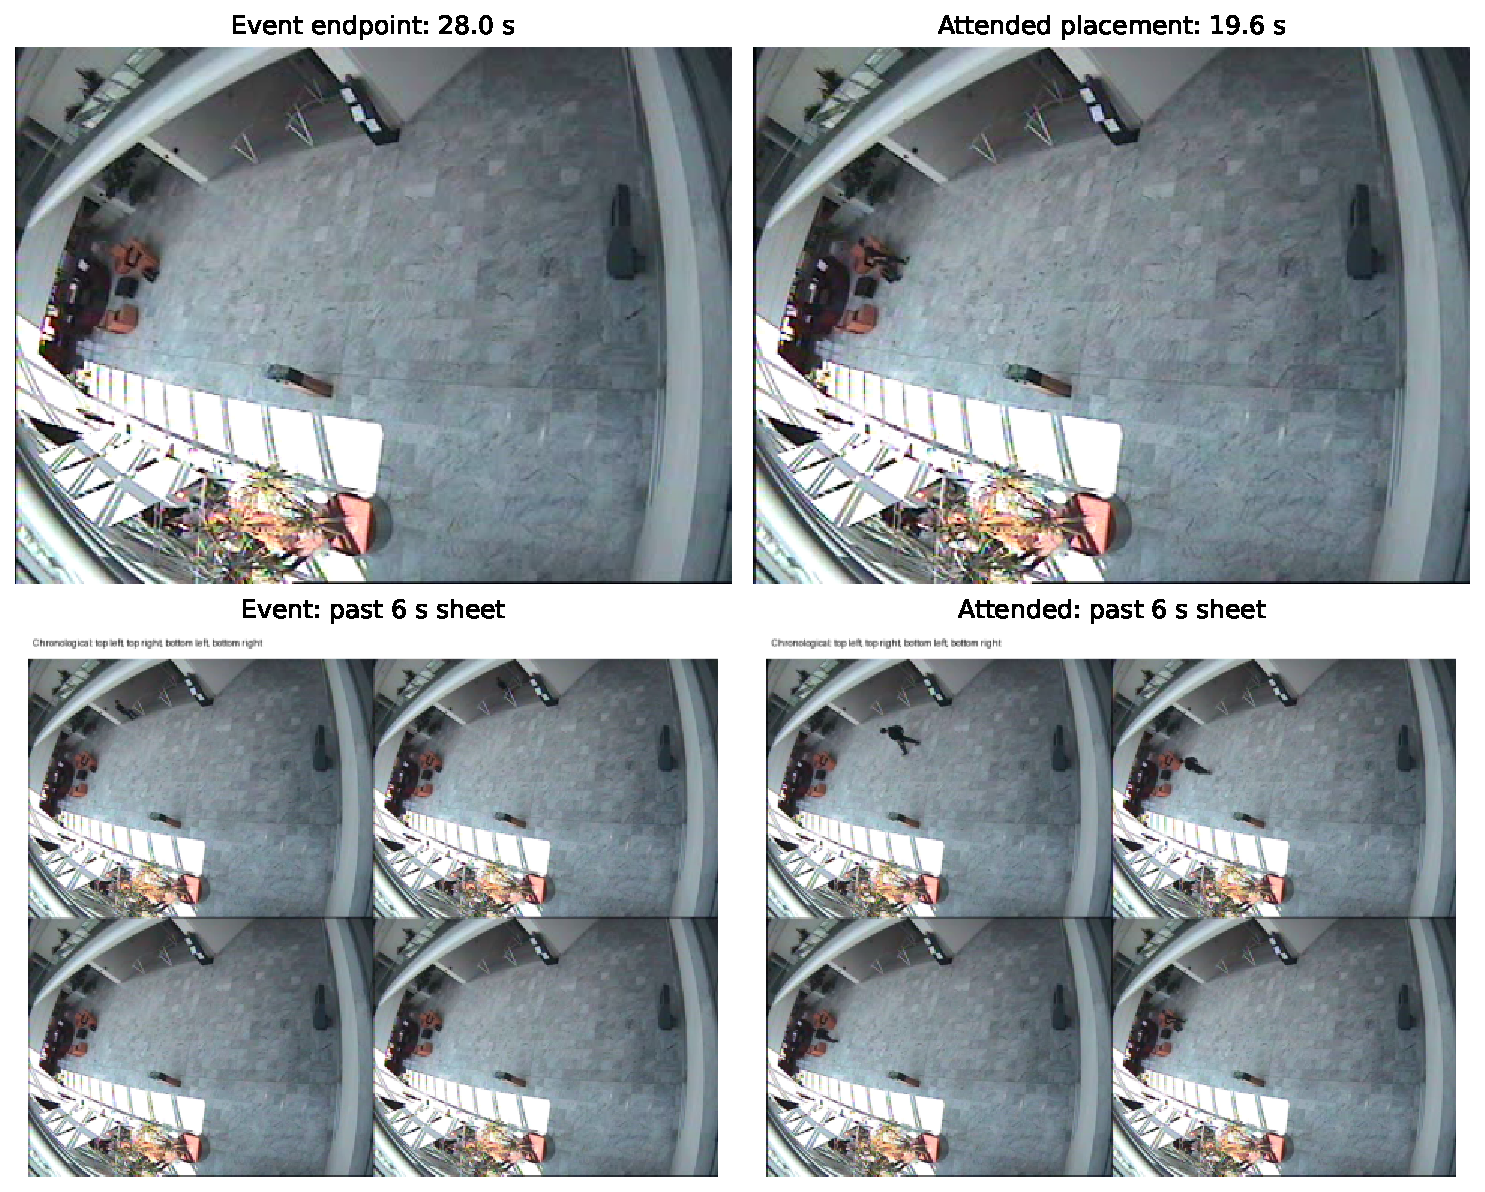
\includegraphics[width=.93\textwidth]{figures/input_examples.pdf}
\caption{Unchanged inputs from the held-out \code{LeftBag_AtChair} recording. The event endpoint is 28.0\,s and the attended-placement control is 19.6\,s. Their past-window sheets contain context ending at those same times. Labels come from the configured sequence review, not a prediction inferred from this figure. Source: CAVIAR project data \cite{caviar}.}
\label{fig:inputs}\end{figure}

\subsection{Fetching and candidates that were not scored}
The unified workflow supports the original Drive corpus and supplementary sources. ABODA publishes eleven abandoned-object scenario videos \cite{aboda}. CAVIAR supplies relevant source video/XML. The D2-CDNet repository provides foreground-segmentation/background-subtraction material \cite{d2}; such masks do not establish ownership or an abandonment event. The two configured Roboflow sources provide suspicious/non-suspicious objects or person/laptop/bag classes \cite{roboflowone,roboflowtwo}. These classes also need event and matched-normal review before task scoring.

This inference invocation used \code{fetch=false}, \code{fetch_drive=false}, \code{skip_prepare=true}, and no review CSV. Thus a claim that this run fetched or human-reviewed all supplementary sources would be unsupported. The local inspection workspace has source receipts, but they are not a substitute for the computation server's receipts. None of ABODA, D2-CDNet or Roboflow contributes a confirmed scored cohort in the provided run. Preparation records 7,200 proxy-development candidates; the current exporter writes only the first 1,000 to its proxy CSV. Neither number denotes scored event examples. The exclusion of posture/person/action proxies explains the missing three anomaly cohorts.

\subsection{Deduplication, grouping and sampling}
Prepared schema 3 addresses aliasing between bundled inputs and freshly decoded copies. Deduplication merges matching byte hashes, exact decoded RGB pixels after EXIF correction, or checksum-qualified CAVIAR source/protocol/time identities. Source times are normalized at microsecond precision. Encoding-only differences therefore do not create extra independent observations. Frame and window protocols stay distinct. Label conflicts cause validation failure, recording aliases are connected into one group, and canonical bundled copies take precedence when equivalent copies exist.

The recorded preparation collected 3,454 confirmed candidate rows, retained 3,350 unique rows and removed 104 aliases. It then retained 308 prepared inputs under sampling caps. These counts describe separate stages: removed aliases are not all exclusions, and the uncapped inference run still operates on a preparation-limited selection. The selected 72 CAVIAR inputs represent 36 endpoint moments in two image protocols. Together with the 236 smoking frames, there are 272 endpoint/frame source observations and 308 image representations; window rows do not add independent event recordings.

Grouping is assigned jointly before protocol-specific inference. Nonhistorical groups are stratified by their label sets, shuffled using seed 42, and approximately 40\% of eligible groups are reserved for test using \code{max(1, round(0.4*n))}. A singleton nonhistorical stratum stays in development. Historical groups also remain development. Within the shuffled prepared rows, the default cap is eight inputs per task/protocol/group/label; CAVIAR generates four times per reviewed interval. This explains why all confirmed candidate files are not inferred even when \code{limit=0}.

For a finite inference cap, the runner uses label-proportional group round-robin selection. This run's zero cap disables that additional subsampling: every available prepared input is selected. Cohort manifests are verified before loading weights. Pixel and source-moment checks reject repeated inputs or cross-split aliases. The audit confirms distinct development/test CAVIAR recording groups and recorded image byte/pixel/source identities for both protocols. It cannot detect every altered or undocumented near duplicate, nor validate inaccessible remote source files.

\section{Experimental implementation and process flow}
\begin{figure}[htbp]\centering
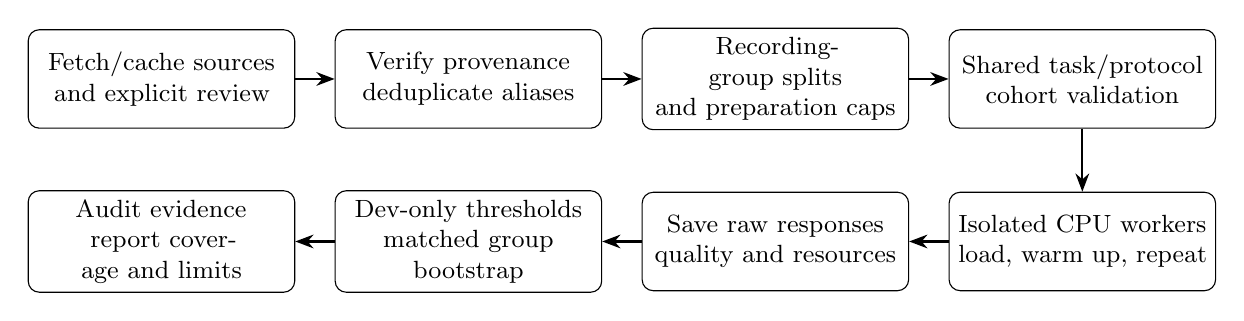
\begin{tikzpicture}[node distance=5mm and 5mm,box/.style={draw,rounded corners,align=center,font=\small,text width=3.15cm,minimum height=1.25cm},arr/.style={-{Stealth},thick}]
\node[box] (a) {Fetch/cache sources\\and explicit review};
\node[box,right=of a] (b) {Verify provenance\\deduplicate aliases};
\node[box,right=of b] (c) {Recording-group splits\\and preparation caps};
\node[box,right=of c] (d) {Shared task/protocol\\cohort validation};
\node[box,below=8mm of d] (f) {Isolated CPU workers\\load, warm up, repeat};
\node[box,left=of f] (g) {Save raw responses\\quality and resources};
\node[box,left=of g] (h) {Dev-only thresholds\\matched group bootstrap};
\node[box,left=of h] (i) {Audit evidence\\report coverage and limits};
\draw[arr] (a)--(b);\draw[arr] (b)--(c);\draw[arr] (c)--(d);\draw[arr] (d)--(f);\draw[arr] (f)--(g);\draw[arr] (g)--(h);\draw[arr] (h)--(i);
\end{tikzpicture}
\caption{Implemented workflow. Source fetching and preparation preceded this inference invocation and were reused. Coverage validation selects available confirmed tasks; missing tasks remain explicitly untested.}
\label{fig:flow}\end{figure}

\subsection{Runner, notebook and worker isolation}
\code{anomaly-eval run} orchestrates preparation, manifest verification, sequential cohort benchmarking, calibration, bootstrap, figures and the report. All models receive the same ordered images, labels and source groups within a task/protocol/split. Development and test are executed as separate benchmark directories. Internally those selected inputs use the worker's \code{test} sample role for measurement; \code{evaluation_split} retains the actual development/test distinction. This internal role does not convert historical development data into a held-out set.

Each model/cohort loads in an isolated process. It writes one flushed JSONL row per measured input/repeat, preserving path, label, source group, pixel hash, origin, protocol, status, prediction, score, raw response, optional token count and latency. Inference exceptions are recorded per input where recoverable. An external supervisor terminates workers that exceed timeout or memory budgets and preserves partial rows. This is why a run-level error can coexist with valid completed cohort results.

The notebook provides a front end to these commands, reads the resulting JSON/CSV and warns against pooling incompatible cohorts. Its default preparation-only path does not run weights until inference is enabled. No saved notebook output establishes additional training, cross-validation or ablation experiments for this run.

\subsection{Common input policy and binary descriptions}
Input loading applies EXIF transpose, converts to RGB, and thumbnails with Lanczos interpolation so the longest dimension does not exceed 768 pixels. The \code{letterbox} policy pads to a square using RGB $(127,127,127)$ without stretching. Native model processing follows. This protects scene edges from a subsequent square center crop, but native input resolution and tokenization remain model-specific. It is not an assertion that each model receives identical final tensor dimensions.

The task-specific normal description is constructed as an ordinary scene with no evidence of the named task. The event description comes from the configuration. Only these two labels are supplied to the evaluated adapters. Labels for irrelevant tasks are omitted. The common text descriptions reduce one source of task-interface variation, but different model families use different native text interfaces. No prompt ensemble, example-based demonstration, object crop, explicit detector or fine-tuning was performed.

The chosen policy is one resource-constrained baseline. A comparison of \code{native} versus \code{letterbox}, more image patches, higher resolutions, longer windows or different prompts would require separate development experiments. General pretrained capabilities do not guarantee performance under the constrained image representation used here.

Recorded native preprocessing is also preserved in each completed summary. MobileCLIP resizes/crops to $256\times256$ with bilinear interpolation and recorded mean zero/std one normalization. SigLIP resizes to $224\times224$, rescales by $1/255$ and normalizes with mean/std 0.5. SmolVLM enables image splitting/padding with a maximum patch edge of 512 and processor longest edge of 768, rescaling by $1/255$ and mean/std 0.5 normalization. MiniCPM records scale resolution 448, patch size 14 and mean/std 0.5; its effective single-slice chat argument overrides the processor's default slice count. These details distinguish the common scene-preservation policy from model-specific tensor construction.

\subsection{Embedding adapters and anomaly scores}
MobileCLIP2 loads the pinned OpenCLIP checkpoint in fp32 on CPU and fuses its convolution branches using timm's reparameterization before timing inference. Text features are computed once during adapter initialization and normalized. For image $x$, normalized image features $v(x)$ and text features $u_k$ give logits
\begin{equation}
 z_k = \exp(a)\,v(x)^T u_k,\quad
 p_k=\frac{\exp(z_k)}{\sum_j\exp(z_j)},\quad
 \hat y=\arg\max_k p_k,\quad s=1-p_{\mathrm{normal}}.
\end{equation}
The scale $a$ is the learned logit scale, not a user-tuned calibration constant. Binary argmax corresponds to the larger of the two relative class scores. The anomaly score is a relative softmax score, not a validated probability of a surveillance event.

SigLIP2 lowercases the text descriptions, pads/truncates to 64 tokens and caches normalized text features. Its native logits include scale and bias:
\begin{equation}
 z_k=\exp(a)\,v(x)^Tu_k+b,\quad
 q_k=\sigma(z_k),\quad \hat y=\arg\max_k z_k,\quad
 s=z_{\mathrm{event}}-z_{\mathrm{normal}}.
\end{equation}
Independent sigmoid values $q_k$ do not sum to one \cite{siglippaper}. A logit margin is therefore used for anomaly ranking and threshold fitting. Raw score magnitudes cannot be compared directly between the two embedding models. Text caching improves repeated inference cost; the model load measurement includes initialization and cached text feature computation.

\subsection{Generative adapters, output constraints and parsing}
SmolVLM uses \code{AutoModelForImageTextToText}, CPU float32 and eager attention. Its native image processor's longest-edge size is bounded to 768. The publisher's chat template formats an image plus the common classification instruction. Generation is greedy, with \code{do_sample=false} and a maximum of 64 new tokens. Only newly generated tokens are decoded for classification; the prompt itself is excluded.

MiniCPM uses the pinned remote-code processor/model, CPU float32 and scaled-dot-product attention. It calls the native \code{chat} interface with the image and the same instruction, cached tokenizer/processor, \code{sampling=false}, one beam, repetition penalty 1.0, 64 new tokens and \code{max_slice_nums=1}. The single-slice constraint bounds work but reduces the model's high-resolution slicing capability relative to unconstrained usage. The processor's advertised slice configuration is not evidence that nine slices were actually used. This is a distinct inference constraint that must accompany any interpretation of MiniCPM's negative results.

The instruction asks for a single JSON label and allows \code{unknown} when duration or ownership evidence is insufficient. Appendix~\ref{app:prompt} preserves the exact template and descriptions. Parsing accepts a case-insensitive whole configured label, optionally quoted or ending in a period, or a JSON object containing a valid \code{label}. It does not search arbitrary prose for a label. An explicit unknown is an abstention; malformed text and ambiguous labels have separate reasons. Raw output is retained. This avoids treating unambiguous capitalized replies as failures while keeping format compliance distinct from event quality.

The earlier pilot exposed case-sensitive rejection of \code{Normal.} and \code{Unattended_items.}, as well as raw/bundled duplicate source moments. Those defects were corrected before this run. They motivate the present exact-label parser and schema-3 alias checks; the old scores are not pooled with these results. Acceptance of plain labels also means that high prediction coverage does not imply compliance with the requested JSON format.

\subsection{Resource settings and measured hardware}
The recorded machine is an AMD Ryzen Threadripper PRO 7975WX with 32 physical and 64 logical CPUs and 257,066.6\,MiB RAM, approximately 251.0\,GiB. The recorded Python is 3.12.3; the platform is Linux 7.0.0-28-generic with glibc 2.39. Runtime versions in completed summaries are torch 2.14.1+cpu, transformers 4.57.1, timm 1.0.30, open\_clip\_torch 3.3.0, Pillow 12.3.0 and psutil 7.2.2.

The runner sets common numerical-library thread variables to 32, PyTorch intra-op threads to 32 and inter-op threads to one. No affinity subset is selected. GPU visibility is disabled and all evaluated tensors/models use CPU. The RSS cap is 24,576\,MiB (24\,GiB). Each image-model job has a 3,600-second timeout including load, warmup and all repeats. A parent also monitors stage process-tree memory. These are execution bounds, not estimates of the target processor's speed.

Evaluation mode uses duty cycle 1.0 and no sample-rate pacing; every completed summary records zero throttle sleep. The one-input/second setting is a budget screen only. It does not slow this evaluation. The deployment mode's cooperative sleeps can pace replay but cannot emulate another processor, impose a hard OS CPU utilization quota, or make a slow model meet a faster arrival rate.

\subsection{Latency, throughput and repeated measurements}
Each model/cohort runs one excluded warmup on the first selected input, followed by three serial passes through the entire cohort. Per-input timing begins before image loading and includes decoding, common/native preprocessing, inference/generation and response parsing. It excludes JSONL writing, supervisor work, initialization, warmup and pacing sleeps. A successful text response that is rejected by the parser still contributes to inference latency; error rows are excluded from the worker's completed-inference latency distribution.

The reported p50/p95 use linear interpolation on sorted measured times. Active throughput divides completed inferences by their summed active latency. Wall throughput divides completed inferences by measured-loop wall time, which includes loop/resource checks and output writing. Model load, warmup and total worker wall time are recorded separately. These are cached-session load timings, not a controlled cold-disk or first-download experiment. RSS is sampled every 50\,ms during load and inference, with additional synchronous checks; instantaneous allocation peaks can be missed.

Quality metrics use repeat zero only, while latency uses all completed repeats. Thus the three passes are timing repetition, not three independent datasets or independent training seeds. The audit observes no label/status changes across available repeats for any model/cohort. No thermal, clock, energy, background-load or thread-count ablation was recorded. Thirty-two configured threads also do not mean exactly thirty-two active cores throughout each model's execution; the CPU-time/wall-time ratio measures an equivalent average.

\section{Evaluation metrics, calibration and uncertainty}
\subsection{Quality and unanswered cases}
For each binary event, let $TP$, $FP$, $FN$ and $TN$ denote detected positives, falsely flagged normals, missed positives and correctly answered normals. Event precision, recall and F1 are
\begin{equation}
 P=\frac{TP}{TP+FP},\quad R=\frac{TP}{N_+},\quad
 F_1=\frac{2TP}{2TP+FP+FN},\quad \mathrm{FPR}=\frac{FP}{N_-}.
\end{equation}
Positive abstentions and errors count in $FN$. Unanswered normal cases are neither true negatives nor false alerts; their number is reported, and they remain in the negative support $N_-$. This makes coverage essential to interpreting FPR and specificity. Overall accuracy including failures is the number of correct valid answers divided by all labeled inputs; conditional accuracy divides by valid answers only. This report uses accuracy including failures in its main tables. The saved field named \code{accuracy} is conditional accuracy and must not be substituted silently when coverage is below one.

Macro F1 averages over ground-truth-supported labels rather than classes a model happened to predict. AUROC uses continuous scores only, with tied scores assigned mean ranks; unsupported or absent continuous scores remain unavailable. Average precision is obtained for continuous-score calibration results. The VLM adapters return categorical labels without event confidence, so no hard-label AUROC, invented probability or token-confidence calibration is provided. Always-normal and always-event baselines give essential class-imbalance context.

\subsection{Development-fitted operating points}
For continuous scores, two operating thresholds are selected on development data and frozen before scoring its paired test cohort. The first maximizes development F1 over precision--recall thresholds; with the implementation's sorted thresholds, ties use the first maximum. The second chooses the smallest candidate threshold satisfying an empirical development FPR no greater than 0.05. Its candidates include every distinct development score and a value immediately above the maximum score. Comparisons use $s\geq\tau$ consistently.

Each CAVIAR development protocol has sixteen normal inputs. Its FPR resolution is $1/16=6.25\%$, so an empirical 5\% budget permits zero development false positives. That is a small-sample constraint, not a population guarantee. Test has twelve normal inputs, yielding 8.33\% per false positive. Test labels never tune a threshold. However, these recordings were part of an already inspected project bundle, and inspection of the present test results will make them development evidence for subsequent changes. A later final deployment claim needs fresh recordings.

\subsection{Group bootstrap and its degeneracy}
The implemented uncertainty calculation resamples source recording groups with replacement, retaining every selected input from each drawn group. Seed 42 and 2,000 shared draws support matched pair differences. Macro classes are fixed from full-cohort support. The central 95\% percentile range is calculated after removing undefined/nonfinite metrics. Pair differences use the same draw and are omitted if either side is undefined.

Each CAVIAR split has three groups and one positive group. The probability that an ordinary three-group bootstrap draw omits that positive group is $(2/3)^3=8/27\approx29.6\%$. The actual saved random stream omits it in 571 of 2,000 draws (28.55\%) for each of the four CAVIAR cohorts. On a negative-only draw, an always-normal model has undefined binary F1, whereas an always-event model has zero F1 because it creates false positives. Consequently, finite-only marginal and paired ranges can condition on different usable draw sets. A nonzero paired interval can coexist with a very weak practical detector and is not proof of broad model superiority.

The audit reproduces the exact saved intervals rather than replacing them with a preferred statistical scheme. Their discrete support and lack of independent positive recordings must accompany the values. No confidence interval estimates generalization to new cameras, and no p-value, multiple-comparison correction, power analysis or repeated-split robustness result is claimed. Before stronger inference, add many independent positive/control recordings and prespecify a class-aware group uncertainty protocol, including how no-positive draws are treated.

\section{Results and evidence audit}
\subsection{Execution status and integrity}
The run has execution status \code{error}, attributable to MiniCPM's smoking timeout. Five benchmark stages were attempted: smoking development, unattended endpoint development/test, and unattended window development/test. Nineteen of twenty model/cohort jobs completed. Planned measured rows total $308\times4\times3=3,696$; 3,684 were saved. Warmup calls are excluded from this total. Stage wall times sum to 7,061.4\,s, approximately 117.7\,min; this excludes preceding preparation and parent-side bootstrap/report time.

The evidence generator performs 139 checks. The single failing check is the planned-cohort completion of MiniCPM smoking. It verifies all complete saved metric dictionaries and p95 values, model/cohort sample lineage, recording/image/source-moment separation, lack of duplicate selected pixels/moments, experiment fingerprints and code hashes. On temporary copies, all four available bootstrap/paired outputs and both calibration files reproduce exactly. SHA-256 inventories confirm that the audit did not change original artifacts.

Eighty-four of the 308 prepared image files can be checked in this inspection workspace against both saved byte and decoded-pixel hashes: all 72 CAVIAR inputs and twelve smoking frames. The remaining 224 smoking files are unavailable locally. Their prediction labels and identities can be audited, but their pixels and source annotation correctness cannot be independently inspected here. The local prepared dataset is an older, different schema-2 bundle with 104 rows; it is not used to replace the server's schema-3 selection. The run folder contains server manifest hashes but not the full server prepared CSVs or fetch receipts, limiting reconstruction of all source-review notes and preparation genealogy.

\subsection{Smoking development discrimination}
MobileCLIP detects two of 116 positives and no normal false positives: precision 1.000, recall 0.017 and F1 0.034. SigLIP predicts normal for all 236 frames, with recall/F1 zero. Their AUROCs are 0.531 and 0.552 respectively, indicating weak development ranking under these descriptions and whole-frame inputs. These are not smoking test results.

SmolVLM detects eleven positives, misses 105 including an unanswered positive, falsely flags nine normals, and correctly answers 109 normals. Two other normals are unanswered. Its event precision is 0.550, recall 0.095, F1 0.162 and FPR 0.075; coverage is $233/236=0.987$. Correct valid answers total 120, so accuracy including failures is $120/236=0.508$, exactly the always-normal accuracy. Conditional accuracy is $120/233=0.515$. The distinction explains why successful execution and some true positives do not yet demonstrate an effective detector.

An always-event smoking baseline has event F1 $232/352=0.659$, but falsely flags every normal input. Its numerically larger F1 is another reason to evaluate a useful precision/recall/false-positive operating point instead of selecting by a single metric. Constant-baseline accuracy depends on each cohort's event prevalence and cannot be compared as a universal performance target.

MiniCPM saves all 236 first-pass rows, all 236 second-pass rows and 224 third-pass rows. Every available response is a valid JSON normal label. It is stopped after 3,601.1\,s for exceeding the 3,600-second timeout. The supervisor preserves sampled peak RSS of 18,407.9\,MiB but cannot obtain the worker's finalized metrics/load/latency summary. Recomputing its complete first pass diagnostically gives zero event recall/F1 and always-normal accuracy; these diagnostics are labeled partial-job evidence in \code{audit.json} and are not represented as a completed benchmark. The original smoking paired bootstrap was refused because the all-model planned cohort was incomplete. Extending its timeout would finish timing coverage, not create an untouched smoking test set.

\subsection{Unattended-item endpoint results}
On development endpoints, MobileCLIP, SigLIP and MiniCPM each predict normal for all twenty inputs; their 80\% accuracy equals the always-normal baseline. SmolVLM predicts the event for every input, yielding event recall 1.000, FPR 1.000 and F1 0.333, equal to the always-event baseline. On sixteen test endpoints, the same constant behaviors yield 75\% always-normal accuracy versus 25\% always-event accuracy and event F1 0.400 for SmolVLM. Constant predictions therefore explain the apparently high accuracy or recall without useful discrimination.

\begin{center}\small
\begin{longtable}{llrrrrrr}
\toprule
Input & Model & TP/4 & FP/12 & Recall & F1 & FPR & Acc. \\
\midrule\endhead
Frame & MobileCLIP2-S2 & 0 & 0 & 0.000 & 0.000 & 0.000 & 0.750 \\
Frame & SigLIP2-B/16 & 0 & 0 & 0.000 & 0.000 & 0.000 & 0.750 \\
Frame & SmolVLM-500M & 4 & 12 & 1.000 & 0.400 & 1.000 & 0.250 \\
Frame & MiniCPM-V 4.0 & 0 & 0 & 0.000 & 0.000 & 0.000 & 0.750 \\
Window & MobileCLIP2-S2 & 1 & 3 & 0.250 & 0.250 & 0.250 & 0.625 \\
Window & SigLIP2-B/16 & 0 & 3 & 0.000 & 0.000 & 0.250 & 0.562 \\
Window & SmolVLM-500M & 3 & 10 & 0.750 & 0.353 & 0.833 & 0.312 \\
Window & MiniCPM-V 4.0 & 0 & 0 & 0.000 & 0.000 & 0.000 & 0.750 \\
\bottomrule
\end{longtable}

\end{center}
The table reports repeat-zero quality; each protocol has four positives and twelve normals. Unsupported events do not appear as zero-valued rows. Full development and resource tables are supplied in the appendices.

\subsection{Past-window results and tradeoffs}
MobileCLIP's test-window confusion counts are $TP=1$, $FP=3$, $FN=3$, $TN=9$, yielding precision/recall/F1 0.250 and FPR 0.250. SigLIP misses all four events and creates three false positives. SmolVLM detects three positives but flags ten of twelve normals, giving recall 0.750, precision 0.231, F1 0.353 and FPR 0.833. MiniCPM remains always normal.

On development windows, neither embedding model detects an event at argmax; MobileCLIP creates four normal false positives and SigLIP one. SmolVLM remains always event; MiniCPM remains always normal. The observed MobileCLIP endpoint-to-window test recall increase from zero to 0.250 is accompanied by extra false alerts and is supported by one correctly flagged moment from one event recording. SmolVLM's window F1 falls below its constant-event endpoint F1. This is mixed, small-sample evidence; it does not establish that temporal reasoning or longer-duration anomaly recognition has been learned.

\begin{figure}[htbp]\centering
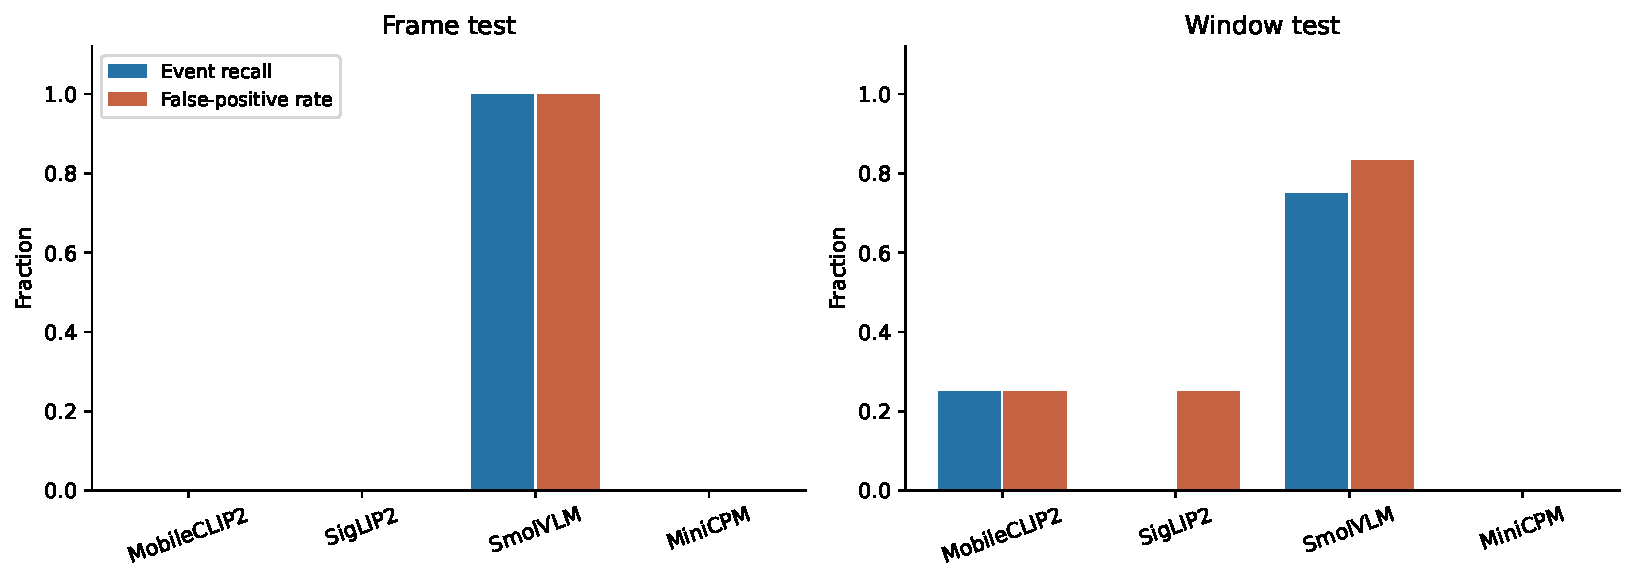
\includegraphics[width=\textwidth]{figures/recall_fpr.pdf}
\caption{Raw unattended-item test recall and false-positive rate. The event and normal denominators are four and twelve per protocol. High recall alone selects the always-event behavior; low false-positive rate alone selects the always-normal behavior. Neither criterion suffices.}
\label{fig:quality}\end{figure}

\subsection{Calibration changes the decision rule, not the visual evidence}
The full-cohort calibration is different from the earlier capped pilot. At MobileCLIP's development-max-F1 endpoint threshold 0.225322, all four test events are detected but eight of twelve normals are falsely flagged, yielding F1 0.500 and FPR 0.667. Its development-FPR threshold 0.396164 yields no false positives and misses all events. SigLIP's maximum-F1 endpoint threshold detects no events and creates five false positives; its FPR-budget rule again predicts all test inputs normal.

For windows, both embedding models' maximum-development-F1 rules flag all sixteen test inputs: recall 1.000, FPR 1.000 and F1 0.400. Their FPR-budget rules each miss all events and falsely flag one normal, giving FPR 0.083. Thus the requested 5\% development budget does not transfer even empirically to test windows. AUROC is 0.354 for MobileCLIP endpoint and 0.438 for its window, and 0.167/0.188 for SigLIP; the score ordering is weak on these test recordings. Threshold tuning alone does not supply reliable ownership evidence.

\begin{figure}[htbp]\centering
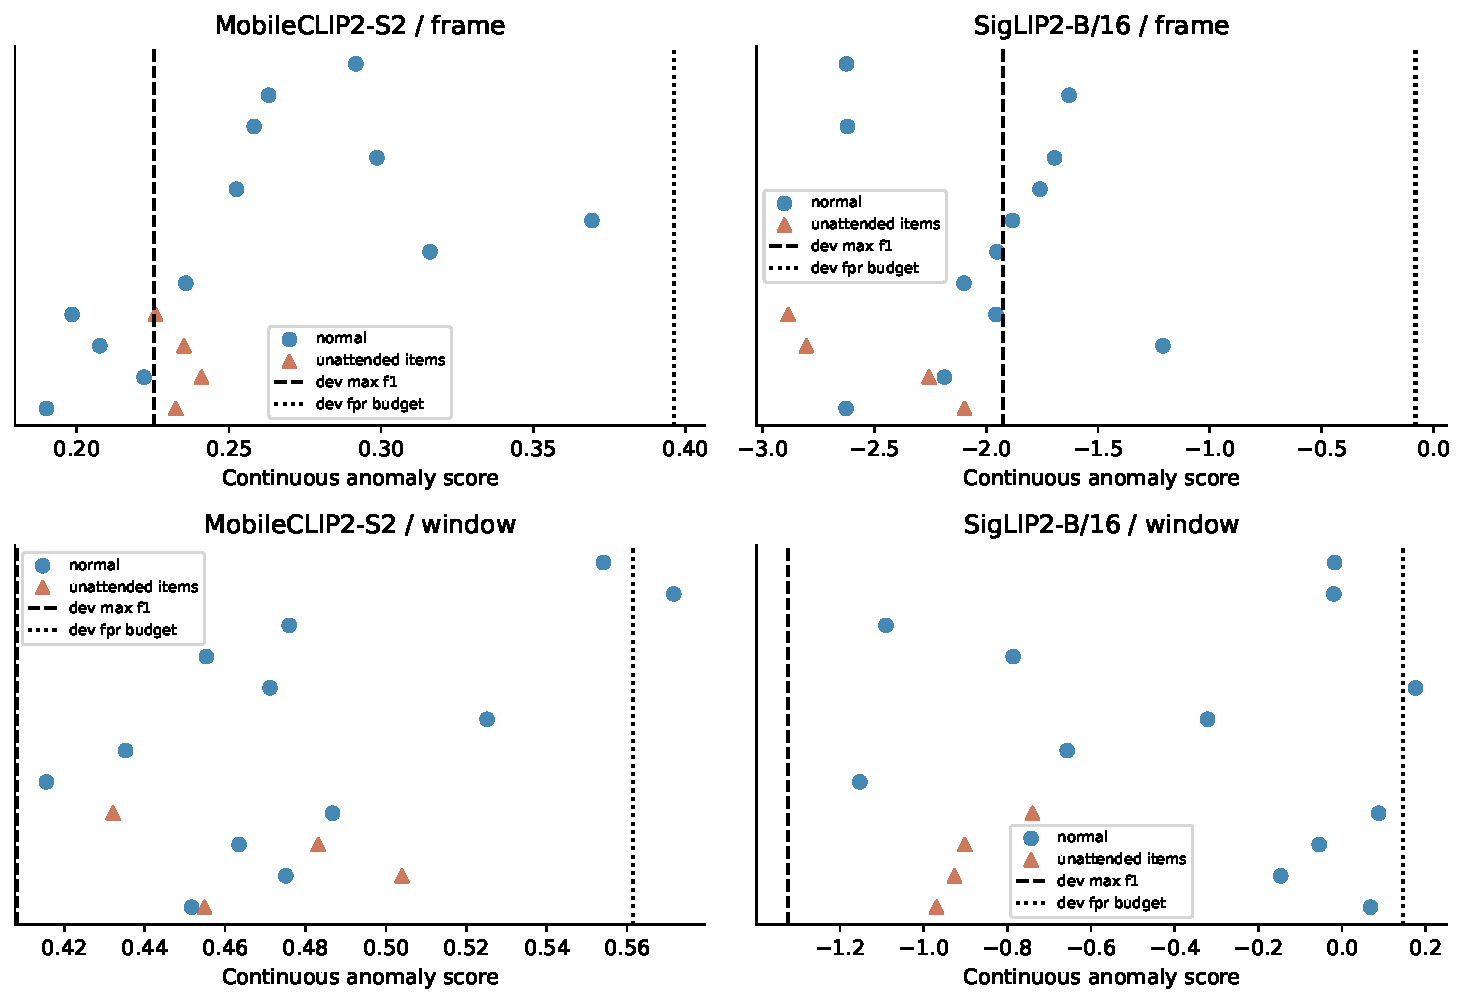
\includegraphics[width=\textwidth]{figures/score_distributions.pdf}
\caption{Observed held-out continuous scores and frozen development thresholds. Vertical offsets separate points visually and have no temporal meaning. Dashed lines maximize development F1; dotted lines impose its empirical FPR budget. MobileCLIP softmax scores and SigLIP logit margins have different scales.}
\label{fig:scores}\end{figure}

\subsection{Output reliability and response diagnostics}
SmolVLM's smoking first pass contains 213 normal labels, twenty smoking labels and three invalid responses. Across repeats, the nine invalid responses are six instances of \code{Lab.} and three instances of \code{Labeling: smoking.}; the latter is not accepted merely because it contains an event word. All valid SmolVLM outputs are plain labels, giving zero JSON-format compliance despite the instruction. No explicit unknown response is observed in this run.

MiniCPM's partial smoking responses are all JSON normal. Its unattended endpoint responses are all plain \code{normal}; development windows are 80\% JSON and test windows are 100\% JSON. These format differences do not improve its event recall. Response-format fractions use returned text responses across measured repeats, while quality uses repeat zero. The full diagnostics table keeps these denominators separate and marks the partial smoking job. Generated token counts are recorded for SmolVLM but unavailable through the MiniCPM string-only chat adapter; the two VLMs therefore have no directly comparable recorded tokens/second result.

\subsection{CPU resource measurements}
On unattended-item test frames, p95 active latency is approximately 0.060\,s for MobileCLIP, 0.044\,s for SigLIP, 3.093\,s for SmolVLM and 2.730\,s for MiniCPM. Corresponding test-window values are 0.065, 0.056, 3.098 and 5.374\,s. The sheet nearly doubles MiniCPM latency despite one-slice inference; the recorded image/processing path makes this a resource observation, not a proved causal attribution to a particular internal operation.

Sampled test RSS is approximately 0.98--1.11\,GiB for MobileCLIP, 1.24\,GiB for SigLIP, 3.11\,GiB for SmolVLM and 17.90--18.38\,GiB for MiniCPM. All are below the run's 24\,GiB cap. The embedding candidates meet the sampled one-input/second budget on this host; both generative candidates exceed a one-second service-time budget. MiniCPM's memory is substantial relative to the intended approximately 32\,GB total system, but no actual target-host end-to-end memory measurement is available.

\begin{figure}[htbp]\centering
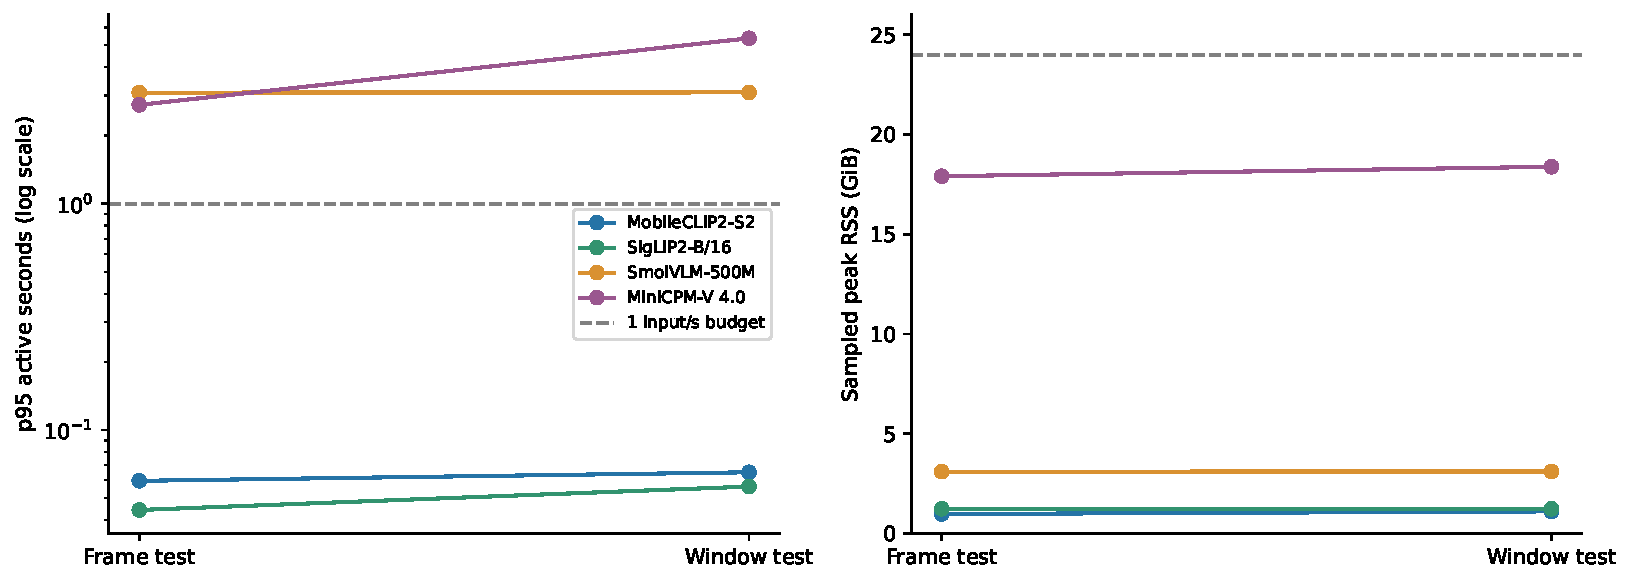
\includegraphics[width=\textwidth]{figures/resources.pdf}
\caption{Measured test p95 latency and sampled worker/process-tree peak RSS. Latency has a logarithmic axis. Dashed lines show the one-input/second and 24\,GiB screens used for this experiment. They exclude camera decoding, queues, alert aggregation and target-host differences.}
\label{fig:resources}\end{figure}

The most computationally economical candidates are therefore worth investigating for improved visual representations or adapted classifiers. That is a feasibility recommendation, not proof that either detects the events adequately. No measured model simultaneously demonstrates useful unattended-item recall, low false-positive rate and deployment-host performance in this evidence set. The data do not justify selecting a generative model simply because its recall or F1 is numerically larger.

\section{Sufficiency, threats to validity and next experiments}
\subsection{What the current evidence can support}
The artifacts are sufficient for a detailed technical report documenting the implemented process, resource-constrained pretrained comparison, observed failure modes, corrected provenance and limitations. The paper has raw per-input evidence, common cohorts, exact settings, checkpoint revisions, preserved failures and reproducible analysis. Negative results are legitimate experimental findings and need not be replaced with an unsupported positive model-selection conclusion.

They are insufficient for a comprehensive five-anomaly, five-model validation or a final deployment-performance paper. An unattended-item sequence holdout exists, but it is a previously inspected, staged, single-camera collection with one positive recording per split. Smoking has larger historical development support, but no untouched test. Three tasks have no confirmed scoring support, and VadCLIP has no executed results. These are evidence gaps rather than low measured scores.

\subsection{Construct, sampling and dependence limitations}
Endpoint state labels and four-frame sheets approximate parts of ownership-related evidence. They do not score continuous abandonment persistence, association of a specific owner, alarm onset/delay or re-attendance over a stream. No loitering duration, littering action boundary or verified sleeping event is evaluated. Current negatives are task-specific and cannot be pooled into a universal normal set without review.

Closely spaced endpoints are correlated; for example four attended test times span only 0.2\,s. Group-level splits address leakage from the same recording but cannot make the four positive endpoints independent events. Frame/window pairs share endpoints and must not be summed as twice the event support. CAVIAR environment similarity also limits generalization across cameras, lighting, crowds, object sizes, occlusion and deployment conditions. Smoking camera/date names provide a grouping approximation whose provenance should be checked against original recording boundaries.

The byte/pixel/source-moment checks resolve exact aliases, including encoding changes, but not all resized, mirrored, cropped or otherwise transformed near duplicates. The source collector's annotation-to-frame label mapping can inherit annotation errors; inaccessible smoking originals prevent a full visual audit. The run contains no reviewer identities, inter-rater agreement, documented adjudication or independently verified event boundary study. Appendix interval notes state precisely the available rationale without claiming more.

\subsection{Model-interface and measurement limitations}
All four candidates are evaluated without anomaly-specific weight adaptation. Text descriptions, letterboxing, a 768-pixel cap, native resizing and bounded generation define one comparison condition, not each model's best achievable operating point. The same sheet format controls access to context but differs from native multi-image/video pathways. MiniCPM's single-slice restriction and SmolVLM's processor limit may suppress useful detail. Successful execution and exact parsing do not validate visual grounding; image-based sanity checks, relevant crops generated by a realistic detector, and deliberate negative controls are still needed.

Three deterministic repeated passes establish local timing/decision behavior, not robustness to random seeds or repeated independent runs. Recorded initialization is not a controlled cold-start benchmark. CPU thread count is high relative to some deployment configurations. The current server's CPU, RAM bandwidth and capacity cannot be extrapolated by throttling to another machine. Latency omits camera decoding, scheduling, queues, detection/tracking, and any alert-state logic; RSS omits a full multi-process live service. Neither alerts/hour, missed event episodes, event delay, sustained camera throughput nor energy is measured.

\subsection{A concrete completion protocol}
A stronger follow-up should preserve the useful common-cohort and provenance machinery while filling the missing evidence:
\begin{enumerate}
\item Specify operational time/ownership criteria and collect or review positive episodes and matched hard controls for each of the five events. Record annotators, review notes, uncertainty and boundaries. Add ABODA or other relevant sequences through explicit review; segmentation/object-class proxies alone remain insufficient.
\item Build source-group-separated development and untouched test sets with substantially more independent events, cameras and conditions. Preserve source genealogy for augmentations and recordings. Freeze final test before model/prompt selection; the present inspected CAVIAR set can serve development work.
\item Verify grounding on easy positive/negative cases and difficult controls, including attended bags, pickup, hand-to-mouth gestures without smoking, temporary presence, lying without the intended event, and disposal into a bin. Report each task's actual support rather than pooling untested tasks.
\item On development only, compare prompts, native versus padded processing, image resolution, detector-generated crops and useful past-window lengths. For temporal events, compare tracking/state logic or a suitably trained video model. Freeze selected settings and thresholds before new test inference.
\item Finish MiniCPM smoking if a complete four-model development resource comparison is needed, using a longer explicit timeout and retaining the original failed run. Running the optional VadCLIP branch is a separate trained smoking study; report encoder cost, adaptation split, supervision differences and any future-context use.
\item Report event precision/recall, false alerts per camera-hour, episode-level detection delay and behavior under uncertain input, alongside per-frame quality. Add a class-aware recording-group uncertainty plan and sensitivity checks with enough groups to support its assumptions.
\item Replay and then run the frozen selected configuration on the actual Ryzen CPU/RAM host. Measure the complete decoder/inference/tracking/alert pipeline for a sustained single stream, including queue growth, dropped frames, warm/cold starts and memory. Throttling is enabled only as a stated pacing experiment.
\end{enumerate}
These are proposed experiments, not completed observations. No assumed improvement from more data, different precision or fine-tuning is entered into the result tables.

\section{Conclusion}
This run strengthens the earlier pilot through schema-3 deduplication, full prepared cohorts, three timing passes and a common past-window protocol. Its completed analysis is reproducible, and its partial timeout is preserved transparently. It provides substantive evidence about the current adapters: embedding models are inexpensive on the measured CPU but have weak event discrimination; generative models are slower and exhibit strong constant-decision behavior on the available unattended-item examples. A higher recall or calibrated F1 can carry unacceptable false-positive behavior.

The appropriate result is a documented screening outcome: no candidate is established as an adequate five-event deployment detector. Further work should be driven by missing event coverage, independent recordings, visual/temporal grounding and actual deployment-host measurements. The detailed tables and audit accompany this conclusion so that a later experiment can change it with evidence rather than inferred capability.

\appendix
\clearpage
\section{Exact classification interface}\label{app:prompt}
The following is the common VLM instruction template from \code{classification_prompt}. The two task-specific description lines replace the bracketed placeholders. SmolVLM wraps this instruction with its chat template; MiniCPM passes it to native chat with an image.
\begin{verbatim}
Classify the visible scene using these definitions:
normal: [TASK-SPECIFIC NORMAL DESCRIPTION]
[TASK]: [EVENT DESCRIPTION]
Choose one best matching label. Use normal only when no defined anomaly
is visible. Use unknown when evidence is insufficient, including missing
evidence of duration or ownership. Reply only with JSON: {"label": "LABEL"}.
Allowed labels: normal, [TASK], unknown.
\end{verbatim}
Line breaks after the description lines above are added for print layout; in the original template the remaining instruction is a continuous string with spaces. Exact definitions are saved in the three \code{*_definitions.json} artifacts. Smoking normal is ``An ordinary scene with no evidence of smoking.'' Its event description is ``A person visibly smoking a cigarette, cigar, or pipe, with a smoking object near the mouth or visible smoke.'' Unattended normal is ``An ordinary scene with no evidence of unattended items.'' Its event description is ``A bag, box, or other personal item apparently left behind without its owner nearby. Ownership and duration require evidence across time.'' The CLIP-family adapters encode these descriptions as text, rather than the generative instruction itself.

\section{Equivalent invocation and evidence files}
The recorded options correspond to the following invocation, with the original server's workspace roots configured. This is a reconstruction of effective settings; a literal top-level shell command was not saved. Model/task choices omitted below are the recorded defaults described in the main text.
\begin{verbatim}
anomaly-eval run --mode evaluation --skip-prepare \
  --threads 32 --repeats 3 --protocols frame window \
  --limit 0 --bootstrap 2000 --seed 42 \
  --timeout-seconds 3600 --max-rss-mb 24576 \
  --image-policy letterbox --max-side 768 --max-new-tokens 64
\end{verbatim}

The recorded input seed is 42, bootstrap draws 2,000, one excluded warmup, no affinity, duty cycle 1.0, no pacing rate, and default development target FPR 0.05. Changing host or runtime libraries creates a new timing condition even if the same images and thresholds are reused.

\begin{longtable}{P{5.4cm}P{9.8cm}}\toprule Artifact & Evidence supplied\\\midrule\endhead
\code{evaluation.json} & Requested/available coverage, execution options and steps, preparation deduplication aliases/counts, code and experiment fingerprints, failures.\\
Cohort \code{run.json} & Host/runtime metadata, ordered sample identities, definitions, selection, image/manifest hashes, actual evaluation split.\\
Model \code{worker_config.json} & Actual planned model and worker settings, including the timed-out job.\\
Model \code{predictions.jsonl} & Raw per-repeat decisions/scores/responses, provenance, statuses and active timing, including preserved partial rows.\\
Model \code{summary.json} & Finalized metrics and resource/format summaries where completed; supervisor error/RSS when interrupted.\\
\code{calibration.json} & Development-selected thresholds, frozen test operating points, AUROC/AP and absence of VLM score calibration.\\
\code{improvements.json} & Group-bootstrap marginal ranges and matched pair differences where the complete planned cohort permits analysis.\\
Logs and \code{comparison.csv} & Worker/stage messages and compact model comparisons; these are supplementary to raw-row checks.\\
\code{paper/audit.json} & Recomputed evidence, 139 checks, unavailable-image counts, source-file SHA inventory, partial-job diagnostics and audit environment.\\
\code{paper/first_pass_cases.jsonl} & A consolidated, derived copy of repeat-zero evidence for inspecting errors without mixing timing repeats.\\
\bottomrule\end{longtable}

Prepared server manifests and source receipts should be retained with this report for full reproduction of annotation/import decisions. Local prepared CSVs have different fingerprints and are not the source for this experiment. Audit recomputation uses a temporary copy and never updates original predictions, summaries, calibration or bootstrap files.

\section{Source intervals and recording support}
The configured CAVIAR intervals below are the actual available review rationale. Each generates four times for each input protocol. ``Event'' means unattended items; normal includes attended placement/retrieval and walking controls.
\small\begin{longtable}{lrrlp{7cm}}
\toprule
Sequence & Start s & End s & Label & Recorded rationale \\
\midrule\endhead
LeftBag & 45.0 & 50.0 & Event & XML object 4 left behind; carrier 3 no longer present; bag persists across this interval. \\
LeftBag & 38.0 & 39.2 & Normal & Bag object 4 remains grouped with depositing carrier 3; attended placement hard negative. \\
LeftBag\_AtChair & 28.0 & 31.0 & Event & Bag object 6 persists after carrier 4 has departed; later retrieval by person 5 is excluded. \\
LeftBag\_AtChair & 19.6 & 19.8 & Normal & Object 6 grouped with carrier 4 during attended placement. \\
LeftBag\_PickedUp & 40.0 & 40.4 & Normal & Object 4 grouped with returning carrier 2; attended retrieval. \\
LeftBag\_PickedUp & 44.0 & 47.0 & Normal & Bag has been picked up; owner walks away with item. \\
Walk1 & 8.0 & 18.0 & Normal & Walking control; no leaving-object role in sequence XML. \\
Walk2 & 8.0 & 30.0 & Normal & Walking control; no leaving-object role in sequence XML. \\
Walk3 & 12.0 & 40.0 & Normal & Walking control; no leaving-object role in sequence XML. \\
\bottomrule
\end{longtable}
\normalsize
\subsection{Selected counts by source group}
\small\begin{longtable}{llrr}
\toprule
Cohort & Source group & Normal & Event \\
\midrule\endhead
Smoking dev & smoke:c1:2025-09-11 & 8 & 3 \\
Smoking dev & smoke:c1:2025-09-14 & 1 & 2 \\
Smoking dev & smoke:c1:2025-09-15 & 7 & 8 \\
Smoking dev & smoke:c1:2025-09-18 & 8 & 7 \\
Smoking dev & smoke:c1:2025-10-07 & 8 & 8 \\
Smoking dev & smoke:c1:2025-10-13 & 8 & 8 \\
Smoking dev & smoke:c1:2025-10-26 & 8 & 8 \\
Smoking dev & smoke:c2:2025-09-11 & 8 & 8 \\
Smoking dev & smoke:c2:2025-09-14 & 8 & 8 \\
Smoking dev & smoke:c2:2025-09-15 & 8 & 8 \\
Smoking dev & smoke:c2:2025-10-07 & 8 & 8 \\
Smoking dev & smoke:c2:2025-10-14 & 8 & 8 \\
Smoking dev & smoke:c2:2025-10-29 & 8 & 8 \\
Smoking dev & smoke:c4:2025-10-16 & 8 & 8 \\
Smoking dev & smoke:c4:2025-10-26 & 8 & 8 \\
Smoking dev & smoke:c4:2025-10-28 & 8 & 8 \\
Frame dev & caviar:LeftBag & 4 & 4 \\
Frame dev & caviar:LeftBag\_PickedUp & 8 & 0 \\
Frame dev & caviar:Walk3 & 4 & 0 \\
Frame test & caviar:LeftBag\_AtChair & 4 & 4 \\
Frame test & caviar:Walk1 & 4 & 0 \\
Frame test & caviar:Walk2 & 4 & 0 \\
Window dev & caviar:LeftBag & 4 & 4 \\
Window dev & caviar:LeftBag\_PickedUp & 8 & 0 \\
Window dev & caviar:Walk3 & 4 & 0 \\
Window test & caviar:LeftBag\_AtChair & 4 & 4 \\
Window test & caviar:Walk1 & 4 & 0 \\
Window test & caviar:Walk2 & 4 & 0 \\
\bottomrule
\end{longtable}
\normalsize

\clearpage\begin{landscape}
\section{Complete categorical quality results}
\small\setlength{\tabcolsep}{4pt}
\begin{longtable}{llrrrrrrrrrrr}
\toprule
Cohort & Model & TP & FP & FN & TN & Acc. & Prec. & Recall & F1 & FPR & Cov. & Macro F1 \\
\midrule\endhead
Smoking dev & MobileCLIP2-S2 & 2 & 0 & 114 & 120 & 0.517 & 1.000 & 0.017 & 0.034 & 0.000 & 1.000 & 0.356 \\
Smoking dev & SigLIP2-B/16 & 0 & 0 & 116 & 120 & 0.508 & 0.000 & 0.000 & 0.000 & 0.000 & 1.000 & 0.337 \\
Smoking dev & SmolVLM-500M & 11 & 9 & 105 & 109 & 0.508 & 0.550 & 0.095 & 0.162 & 0.075 & 0.987 & 0.408 \\
Smoking dev & MiniCPM-V 4.0$^\dagger$ & -- & -- & -- & -- & -- & -- & -- & -- & -- & -- & -- \\
Frame dev & MobileCLIP2-S2 & 0 & 0 & 4 & 16 & 0.800 & 0.000 & 0.000 & 0.000 & 0.000 & 1.000 & 0.444 \\
Frame dev & SigLIP2-B/16 & 0 & 0 & 4 & 16 & 0.800 & 0.000 & 0.000 & 0.000 & 0.000 & 1.000 & 0.444 \\
Frame dev & SmolVLM-500M & 4 & 16 & 0 & 0 & 0.200 & 0.200 & 1.000 & 0.333 & 1.000 & 1.000 & 0.167 \\
Frame dev & MiniCPM-V 4.0 & 0 & 0 & 4 & 16 & 0.800 & 0.000 & 0.000 & 0.000 & 0.000 & 1.000 & 0.444 \\
Frame test & MobileCLIP2-S2 & 0 & 0 & 4 & 12 & 0.750 & 0.000 & 0.000 & 0.000 & 0.000 & 1.000 & 0.429 \\
Frame test & SigLIP2-B/16 & 0 & 0 & 4 & 12 & 0.750 & 0.000 & 0.000 & 0.000 & 0.000 & 1.000 & 0.429 \\
Frame test & SmolVLM-500M & 4 & 12 & 0 & 0 & 0.250 & 0.250 & 1.000 & 0.400 & 1.000 & 1.000 & 0.200 \\
Frame test & MiniCPM-V 4.0 & 0 & 0 & 4 & 12 & 0.750 & 0.000 & 0.000 & 0.000 & 0.000 & 1.000 & 0.429 \\
Window dev & MobileCLIP2-S2 & 0 & 4 & 4 & 12 & 0.600 & 0.000 & 0.000 & 0.000 & 0.250 & 1.000 & 0.375 \\
Window dev & SigLIP2-B/16 & 0 & 1 & 4 & 15 & 0.750 & 0.000 & 0.000 & 0.000 & 0.062 & 1.000 & 0.429 \\
Window dev & SmolVLM-500M & 4 & 16 & 0 & 0 & 0.200 & 0.200 & 1.000 & 0.333 & 1.000 & 1.000 & 0.167 \\
Window dev & MiniCPM-V 4.0 & 0 & 0 & 4 & 16 & 0.800 & 0.000 & 0.000 & 0.000 & 0.000 & 1.000 & 0.444 \\
Window test & MobileCLIP2-S2 & 1 & 3 & 3 & 9 & 0.625 & 0.250 & 0.250 & 0.250 & 0.250 & 1.000 & 0.500 \\
Window test & SigLIP2-B/16 & 0 & 3 & 4 & 9 & 0.562 & 0.000 & 0.000 & 0.000 & 0.250 & 1.000 & 0.360 \\
Window test & SmolVLM-500M & 3 & 10 & 1 & 2 & 0.312 & 0.231 & 0.750 & 0.353 & 0.833 & 1.000 & 0.310 \\
Window test & MiniCPM-V 4.0 & 0 & 0 & 4 & 12 & 0.750 & 0.000 & 0.000 & 0.000 & 0.000 & 1.000 & 0.429 \\
\bottomrule
\end{longtable}

\normalsize
Accuracy includes unanswered inputs. Cov. is valid prediction coverage. F1 is event F1, rather than macro F1. Values use repeat zero. $\dagger$ indicates the timed-out smoking job: finalized metrics are unavailable; complete first-pass diagnostics are in the audit and are not substituted here. For SmolVLM smoking, two unanswered normals are outside TN/FP and one unanswered positive is in FN.
\end{landscape}

\begin{landscape}
\section{Complete CPU resource results}
\small\setlength{\tabcolsep}{5pt}
\begin{longtable}{llrrrrrrr}
\toprule
Cohort & Model & Load s & Warm s & p50 s & p95 s & Active/s & CPU eq. & GiB \\
\midrule\endhead
Smoking dev & MobileCLIP2-S2 & 3.194 & 0.091 & 0.053 & 0.059 & 18.533 & 31.2 & 0.97 \\
Smoking dev & SigLIP2-B/16 & 4.794 & 0.037 & 0.044 & 0.048 & 23.080 & 29.6 & 1.25 \\
Smoking dev & SmolVLM-500M & 4.471 & 2.604 & 2.510 & 2.629 & 0.398 & 22.7 & 3.09 \\
Smoking dev & MiniCPM-V 4.0 & -- & -- & -- & -- & -- & -- & 17.98 \\
Frame dev & MobileCLIP2-S2 & 3.177 & 0.096 & 0.052 & 0.056 & 19.258 & 31.4 & 0.98 \\
Frame dev & SigLIP2-B/16 & 4.813 & 0.046 & 0.042 & 0.045 & 24.449 & 30.0 & 1.24 \\
Frame dev & SmolVLM-500M & 4.550 & 2.975 & 2.934 & 3.058 & 0.340 & 23.0 & 3.11 \\
Frame dev & MiniCPM-V 4.0 & 5.653 & 2.611 & 2.511 & 2.695 & 0.395 & 26.0 & 17.88 \\
Frame test & MobileCLIP2-S2 & 3.321 & 0.093 & 0.054 & 0.060 & 18.445 & 31.4 & 0.98 \\
Frame test & SigLIP2-B/16 & 5.085 & 0.052 & 0.037 & 0.044 & 26.256 & 30.1 & 1.24 \\
Frame test & SmolVLM-500M & 4.509 & 2.902 & 2.967 & 3.093 & 0.337 & 22.9 & 3.11 \\
Frame test & MiniCPM-V 4.0 & 5.816 & 2.582 & 2.514 & 2.730 & 0.393 & 26.0 & 17.90 \\
Window dev & MobileCLIP2-S2 & 3.284 & 0.099 & 0.063 & 0.068 & 15.840 & 27.6 & 1.17 \\
Window dev & SigLIP2-B/16 & 4.884 & 0.054 & 0.051 & 0.057 & 19.468 & 24.5 & 1.24 \\
Window dev & SmolVLM-500M & 4.514 & 2.974 & 3.007 & 3.124 & 0.333 & 22.7 & 3.11 \\
Window dev & MiniCPM-V 4.0 & 5.752 & 5.109 & 5.105 & 5.322 & 0.216 & 18.6 & 18.42 \\
Window test & MobileCLIP2-S2 & 3.271 & 0.097 & 0.061 & 0.065 & 16.356 & 27.6 & 1.11 \\
Window test & SigLIP2-B/16 & 5.127 & 0.063 & 0.053 & 0.056 & 19.209 & 25.3 & 1.24 \\
Window test & SmolVLM-500M & 4.492 & 2.931 & 2.914 & 3.098 & 0.347 & 22.7 & 3.11 \\
Window test & MiniCPM-V 4.0 & 5.919 & 5.189 & 5.201 & 5.374 & 0.192 & 17.6 & 18.38 \\
\bottomrule
\end{longtable}

\normalsize
Latency and active/s exclude deliberate sleep, which is zero in completed jobs. CPU eq. is measured process CPU seconds divided by measured loop wall seconds, rather than a percentage or physical-core allocation. RSS is sampled worker/process-tree peak and GiB uses $2^{30}$ bytes. Loading includes adapter initialization/cached text features. Warmup is excluded from measured rows. MiniCPM smoking retains supervisor RSS but lacks finalized load/warmup/latency/throughput data.
\end{landscape}

\begin{landscape}
\subsection{Additional timing and throughput fields}
\small\setlength{\tabcolsep}{5pt}
\begin{longtable}{llrrrrr}
\toprule
Cohort & Model & Mean s & Wall/s & Loop wall s & Loop CPU s & Worker wall s \\
\midrule\endhead
Smoking dev & MobileCLIP2-S2 & 0.054 & 18.319 & 38.648 & 1204.763 & 42.585 \\
Smoking dev & SigLIP2-B/16 & 0.043 & 22.739 & 31.136 & 922.047 & 36.619 \\
Smoking dev & SmolVLM-500M & 2.511 & 0.398 & 1778.488 & 40410.308 & 1786.204 \\
Smoking dev & MiniCPM-V 4.0 & -- & -- & -- & -- & 3601.092 \\
Frame dev & MobileCLIP2-S2 & 0.052 & 19.065 & 3.147 & 98.781 & 7.078 \\
Frame dev & SigLIP2-B/16 & 0.041 & 24.132 & 2.486 & 74.595 & 7.971 \\
Frame dev & SmolVLM-500M & 2.941 & 0.340 & 176.467 & 4052.528 & 184.611 \\
Frame dev & MiniCPM-V 4.0 & 2.530 & 0.395 & 151.816 & 3943.811 & 160.748 \\
Frame test & MobileCLIP2-S2 & 0.054 & 18.258 & 2.629 & 82.577 & 6.760 \\
Frame test & SigLIP2-B/16 & 0.038 & 25.884 & 1.854 & 55.854 & 7.614 \\
Frame test & SmolVLM-500M & 2.967 & 0.337 & 142.452 & 3265.120 & 150.513 \\
Frame test & MiniCPM-V 4.0 & 2.544 & 0.393 & 122.149 & 3174.857 & 131.185 \\
Window dev & MobileCLIP2-S2 & 0.063 & 15.698 & 3.822 & 105.592 & 7.870 \\
Window dev & SigLIP2-B/16 & 0.051 & 19.257 & 3.116 & 76.191 & 8.678 \\
Window dev & SmolVLM-500M & 3.000 & 0.333 & 180.040 & 4078.881 & 188.164 \\
Window dev & MiniCPM-V 4.0 & 4.637 & 0.216 & 278.245 & 5171.233 & 289.752 \\
Window test & MobileCLIP2-S2 & 0.061 & 16.212 & 2.961 & 81.684 & 6.986 \\
Window test & SigLIP2-B/16 & 0.052 & 19.000 & 2.526 & 63.827 & 8.370 \\
Window test & SmolVLM-500M & 2.885 & 0.346 & 138.529 & 3148.368 & 146.597 \\
Window test & MiniCPM-V 4.0 & 5.206 & 0.192 & 249.929 & 4391.690 & 261.757 \\
\bottomrule
\end{longtable}

\normalsize
Mean latency uses completed inference rows. Wall/s includes measured-loop bookkeeping but excludes initialization/warmup. Loop wall and CPU values describe three passes through each prepared cohort. Worker wall additionally includes loading and other worker overhead. The timed-out MiniCPM job retains only its supervisor wall duration and sampled RSS. Timing repeats are not additional independent quality observations.
\end{landscape}

\begin{landscape}
\section{Frozen development calibration on test}
\small\setlength{\tabcolsep}{4pt}
\begin{longtable}{lllrrrrrrrrr}
\toprule
Protocol & Model & Rule & Threshold & TP & FP & FN & TN & Recall & F1 & FPR & AP \\
\midrule\endhead
Frame test & MobileCLIP2-S2 & Max dev F1 & 0.225322 & 4 & 8 & 0 & 4 & 1.000 & 0.500 & 0.667 & 0.233 \\
Frame test & MobileCLIP2-S2 & Dev FPR budget & 0.396164 & 0 & 0 & 4 & 12 & 0.000 & 0.000 & 0.000 & 0.233 \\
Frame test & SigLIP2-B/16 & Max dev F1 & -1.925811 & 0 & 5 & 4 & 7 & 0.000 & 0.000 & 0.417 & 0.189 \\
Frame test & SigLIP2-B/16 & Dev FPR budget & -0.079415 & 0 & 0 & 4 & 12 & 0.000 & 0.000 & 0.000 & 0.189 \\
Window test & MobileCLIP2-S2 & Max dev F1 & 0.408146 & 4 & 12 & 0 & 0 & 1.000 & 0.400 & 1.000 & 0.275 \\
Window test & MobileCLIP2-S2 & Dev FPR budget & 0.561465 & 0 & 1 & 4 & 11 & 0.000 & 0.000 & 0.083 & 0.275 \\
Window test & SigLIP2-B/16 & Max dev F1 & -1.323678 & 4 & 12 & 0 & 0 & 1.000 & 0.400 & 1.000 & 0.196 \\
Window test & SigLIP2-B/16 & Dev FPR budget & 0.144867 & 0 & 1 & 4 & 11 & 0.000 & 0.000 & 0.083 & 0.196 \\
\bottomrule
\end{longtable}

\normalsize
Each rule uses sixteen development negatives and is evaluated on four positives/twelve negatives. AP is average precision, not an oracle thresholded F1. A development 5\% FPR target permits zero false positives at 6.25\% resolution. VLMs have no continuous-score threshold or AP/AUROC in this implementation. Rounded thresholds are for presentation; saved floating-point values were used for verification.
\end{landscape}

\clearpage\section{Recorded bootstrap and matched differences}
\small\begin{longtable}{llrlrl}
\toprule
Cohort & Model & F1 & 95\% range & AUROC & 95\% range \\
\midrule\endhead
Frame dev & MobileCLIP2-S2 & 0.000 & [0.000, 0.000] & 0.484 & [0.250, 0.525] \\
Frame dev & SigLIP2-B/16 & 0.000 & [0.000, 0.000] & 0.547 & [0.312, 0.613] \\
Frame dev & SmolVLM-500M & 0.333 & [0.000, 0.667] & -- & -- \\
Frame dev & MiniCPM-V 4.0 & 0.000 & [0.000, 0.000] & -- & -- \\
Frame test & MobileCLIP2-S2 & 0.000 & [0.000, 0.000] & 0.354 & [0.292, 0.750] \\
Frame test & SigLIP2-B/16 & 0.000 & [0.000, 0.000] & 0.167 & [0.125, 0.167] \\
Frame test & SmolVLM-500M & 0.400 & [0.000, 0.667] & -- & -- \\
Frame test & MiniCPM-V 4.0 & 0.000 & [0.000, 0.000] & -- & -- \\
Window dev & MobileCLIP2-S2 & 0.000 & [0.000, 0.000] & 0.297 & [0.167, 0.500] \\
Window dev & SigLIP2-B/16 & 0.000 & [0.000, 0.000] & 0.250 & [0.000, 0.500] \\
Window dev & SmolVLM-500M & 0.333 & [0.000, 0.667] & -- & -- \\
Window dev & MiniCPM-V 4.0 & 0.000 & [0.000, 0.000] & -- & -- \\
Window test & MobileCLIP2-S2 & 0.250 & [0.000, 0.333] & 0.438 & [0.375, 0.458] \\
Window test & SigLIP2-B/16 & 0.000 & [0.000, 0.000] & 0.188 & [0.000, 0.375] \\
Window test & SmolVLM-500M & 0.353 & [0.000, 0.545] & -- & -- \\
Window test & MiniCPM-V 4.0 & 0.000 & [0.000, 0.000] & -- & -- \\
\bottomrule
\end{longtable}
\normalsize
The central ranges omit undefined/nonfinite draws; they are exploratory three-recording estimates. All four cohorts omit the positive recording in 571 draws. Categorical zero-F1 intervals are properties of constant decisions on the observed data, not certainty about population recall. Smoking has no saved all-model bootstrap because of the incomplete MiniCPM job.
\clearpage\subsection{Paired event-F1 differences}
\small\begin{longtable}{llrl}
\toprule
Cohort & Model difference & $\Delta$F1 & 95\% range \\
\midrule\endhead
Frame dev & MobileCLIP2-S2 - SigLIP2-B/16 & 0.000 & [0.000, 0.000] \\
Frame dev & MobileCLIP2-S2 - SmolVLM-500M & -0.333 & [-0.667, -0.286] \\
Frame dev & MobileCLIP2-S2 - MiniCPM-V 4.0 & 0.000 & [0.000, 0.000] \\
Frame dev & SigLIP2-B/16 - SmolVLM-500M & -0.333 & [-0.667, -0.286] \\
Frame dev & SigLIP2-B/16 - MiniCPM-V 4.0 & 0.000 & [0.000, 0.000] \\
Frame dev & SmolVLM-500M - MiniCPM-V 4.0 & 0.333 & [0.286, 0.667] \\
Frame test & MobileCLIP2-S2 - SigLIP2-B/16 & 0.000 & [0.000, 0.000] \\
Frame test & MobileCLIP2-S2 - SmolVLM-500M & -0.400 & [-0.667, -0.400] \\
Frame test & MobileCLIP2-S2 - MiniCPM-V 4.0 & 0.000 & [0.000, 0.000] \\
Frame test & SigLIP2-B/16 - SmolVLM-500M & -0.400 & [-0.667, -0.400] \\
Frame test & SigLIP2-B/16 - MiniCPM-V 4.0 & 0.000 & [0.000, 0.000] \\
Frame test & SmolVLM-500M - MiniCPM-V 4.0 & 0.400 & [0.400, 0.667] \\
Window dev & MobileCLIP2-S2 - SigLIP2-B/16 & 0.000 & [0.000, 0.000] \\
Window dev & MobileCLIP2-S2 - SmolVLM-500M & -0.333 & [-0.667, 0.000] \\
Window dev & MobileCLIP2-S2 - MiniCPM-V 4.0 & 0.000 & [0.000, 0.000] \\
Window dev & SigLIP2-B/16 - SmolVLM-500M & -0.333 & [-0.667, -0.286] \\
Window dev & SigLIP2-B/16 - MiniCPM-V 4.0 & 0.000 & [0.000, 0.000] \\
Window dev & SmolVLM-500M - MiniCPM-V 4.0 & 0.333 & [0.286, 0.667] \\
Window test & MobileCLIP2-S2 - SigLIP2-B/16 & 0.250 & [0.000, 0.333] \\
Window test & MobileCLIP2-S2 - SmolVLM-500M & -0.103 & [-0.212, 0.000] \\
Window test & MobileCLIP2-S2 - MiniCPM-V 4.0 & 0.250 & [0.250, 0.333] \\
Window test & SigLIP2-B/16 - SmolVLM-500M & -0.353 & [-0.545, 0.000] \\
Window test & SigLIP2-B/16 - MiniCPM-V 4.0 & 0.000 & [0.000, 0.000] \\
Window test & SmolVLM-500M - MiniCPM-V 4.0 & 0.353 & [0.353, 0.545] \\
\bottomrule
\end{longtable}
\normalsize
These are differences within a cohort, not across frame/window protocols. A positive difference can reflect an always-event model compared with an always-normal model and must be considered with false positives. Different undefined-draw patterns limit interpretation of the finite-only pair ranges. No statistical significance or global model ranking is asserted.

\clearpage\section{Response formats and decision counts}
\small\begin{longtable}{llrrP{5.0cm}}
\toprule
Cohort & Model & Rows & JSON frac. & First-pass decisions \\
\midrule\endhead
Smoking dev & SmolVLM-500M & 708 & 0.000 & normal:213, smoking:20, unanswered:3 \\
Smoking dev & MiniCPM-V 4.0 & 696 & 1.000 & normal:236 \\
Frame dev & SmolVLM-500M & 60 & 0.000 & unattended\_items:20 \\
Frame dev & MiniCPM-V 4.0 & 60 & 0.000 & normal:20 \\
Frame test & SmolVLM-500M & 48 & 0.000 & unattended\_items:16 \\
Frame test & MiniCPM-V 4.0 & 48 & 0.000 & normal:16 \\
Window dev & SmolVLM-500M & 60 & 0.000 & unattended\_items:20 \\
Window dev & MiniCPM-V 4.0 & 60 & 0.800 & normal:20 \\
Window test & SmolVLM-500M & 48 & 0.000 & normal:3, unattended\_items:13 \\
Window test & MiniCPM-V 4.0 & 48 & 1.000 & normal:16 \\
\bottomrule
\end{longtable}
\normalsize
Row counts include measured repeats, whereas first-pass decisions describe quality support once. JSON fraction counts valid structured labels including explicit structured unknowns, if present, over returned text responses. Malformed text stays invalid even when it includes a class word. MiniCPM smoking has only 696 of 708 planned rows; its available first pass is complete. No explicit unknown was observed. Non-generative models do not have a text format-compliance measure.

\section{Evidence sufficiency matrix}
\begin{longtable}{P{4.2cm}P{5.2cm}P{5.5cm}}\toprule Claim area & Available evidence & Remaining limitation\\\midrule\endhead
Methods/process & Matched source hashes, code, definitions, sample identities and commands & No preregistration or complete human decision diary\\
Four pretrained models & Twenty requested jobs, nineteen complete & MiniCPM smoking timing incomplete\\
Smoking quality & 236 labeled development frames, sixteen source groups & No untouched smoking test; 224 files unavailable locally\\
Unattended-item quality & Frame/window dev/test; attended and retrieval controls & One positive recording per split, staged common camera\\
Other three anomalies & Names, definitions, proxy candidates & No confirmed event/normal scored cohorts\\
VadCLIP & Optional implementation and published method & No executed result in this folder\\
Threshold operation & Development-only fitting and complete test calibration & Too few normals for a reliable 5\% population FPR\\
Uncertainty & Reproduced 2,000 recording-group draws and pair results & Sparse groups, class-absent draws and finite-only conditioning\\
Resources & Three repeated measured passes, RSS, host/thread versions & No target Ryzen run, energy, sustained stream or queue measurement\\
Live event detection & Past-only image-sheet protocol & No alerts/hour, event delay, tracking or continuous episode scoring\\
\bottomrule\end{longtable}

\clearpage
\begin{thebibliography}{99}
\bibitem{clip} A. Radford et al. \emph{Learning Transferable Visual Models From Natural Language Supervision}. 2021. \url{https://arxiv.org/abs/2103.00020}.
\bibitem{mobilepaper} F. Faghri et al. \emph{MobileCLIP2: Improving Multi-Modal Reinforced Training}. 2025. \url{https://arxiv.org/abs/2508.20691}.
\bibitem{mobilecard} PyTorch Image Models. \emph{MobileCLIP2-S2-OpenCLIP model card}, adapted from Apple's checkpoint. \url{https://huggingface.co/timm/MobileCLIP2-S2-OpenCLIP}.
\bibitem{siglippaper} X. Zhai et al. \emph{Sigmoid Loss for Language Image Pre-Training}. 2023. \url{https://arxiv.org/abs/2303.15343}.
\bibitem{siglip2paper} M. Tschannen et al. \emph{SigLIP 2: Multilingual Vision-Language Encoders with Improved Semantic Understanding, Localization, and Dense Features}. 2025. \url{https://arxiv.org/abs/2502.14786}.
\bibitem{siglipcard} Google. \emph{SigLIP2-base-patch16-224 model card}. \url{https://huggingface.co/google/siglip2-base-patch16-224}.
\bibitem{smolpaper} A. Marafioti et al. \emph{SmolVLM: Redefining Small and Efficient Multimodal Models}. 2025. \url{https://arxiv.org/abs/2504.05299}.
\bibitem{smolcard} HuggingFaceTB. \emph{SmolVLM-500M-Instruct model card}. \url{https://huggingface.co/HuggingFaceTB/SmolVLM-500M-Instruct}.
\bibitem{minicard} OpenBMB. \emph{MiniCPM-V 4.0 model card}. \url{https://huggingface.co/openbmb/MiniCPM-V-4}.
\bibitem{vadclip} P. Wu et al. \emph{VadCLIP: Adapting Vision-Language Models for Weakly Supervised Video Anomaly Detection}. 2023. \url{https://arxiv.org/abs/2308.11681}.
\bibitem{caviar} CAVIAR project. \emph{Context Aware Vision using Image-based Active Recognition: project and datasets}. \url{https://homepages.inf.ed.ac.uk/rbf/CAVIAR/}. Original source dataset link: \url{https://groups.inf.ed.ac.uk/vision/DATASETS/CAVIAR/CAVIARDATA1/}.
\bibitem{aboda} K. Lin. \emph{ABODA: Abandoned Object Dataset}. \url{https://github.com/kevinlin311tw/ABODA}.
\bibitem{d2} T. Akhund. \emph{D2-CDNet dataset repository}. \url{https://huggingface.co/datasets/tauseefakhund/D2-CDNet}.
\bibitem{roboflowone} Roboflow Universe. \emph{Abandoned Object Detection source configured by this project}. \url{https://universe.roboflow.com/abandoned-object/abandoned-object-detection-9fijk}.
\bibitem{roboflowtwo} Roboflow Universe. \emph{Abandoned source configured by this project}. \url{https://universe.roboflow.com/getting/abandoned-w7arq}.
\end{thebibliography}
External model/paper/project references were checked on 12 October 2026. The CAVIAR dataset endpoint was not retrievable through the web inspection tool on that date; locally available curated inputs and the recorded source identities support the dataset-specific analysis. Roboflow links identify configured candidates, not scored data or verified access. Local original experiment artifacts and the source implementation are the primary evidence for all numerical results in this report.
\end{document}
